\documentclass[a4paper]{article}

\usepackage[francais]{babel}
\usepackage[utf8]{inputenc}
\usepackage[T1]{fontenc}
\usepackage{graphicx}
\usepackage{tikz}
\usepackage{hyperref}
\usepackage{xcolor}
\hypersetup{
    colorlinks,
    linkcolor={blue!50!black},
    citecolor={blue!50!black},
    urlcolor={blue!80!black}
}

\bibliographystyle{plain-fr}

\title{\textbf{Rapport de Conception} \\ Création d'un jeu SmallWorld}

\author{Laura \textsc{Guillemot}, Thibault \textsc{Rapin}\\
		\\
        Encadrant : Eric \textsc{Anquetil}, Ferran \textsc{Argelaguet},\\
        Arnaud \textsc{Blouin}, Grégoire \textsc{Richard}, Maud \textsc{Marchal}}         


\begin{document}


\maketitle
\thispagestyle{empty}

\newpage
\tableofcontents
\newpage

\section*{Introduction}
\addcontentsline{toc}{section}{Introduction} 

Le jeu Small Word est un jeu tour-par-tour où chaque joueur dirige un peuple. Le but est de gérer des unités sur une carte pour obtenir le plus de points possibles à la fin d’un certain nombre de tours.

Ce rapport présente donc notre solution de modélisation du jeu. Il sera illustré à l’aide de différents diagrammes UML que nous expliciterons.



\section{Diagrammes de cas d'utilisation}

\subsection{Cas de lancement d’une partie}

Lorsque le joueur souhaite lancer une partie, il a deux possibilités (figure \ref{usecasecreate}) : il peut lancer une partie déjà enregistrée ou il peut créer une nouvelle partie.
S’il choisit la première option, c’est-à-dire s’il décide de lancer une partie enregistrée, il devra en plus sélectionner la partie qu’il souhaite charger parmi les parties existantes.
Si l’utilisateur souhaite lancer une nouvelle partie, il devra alors créer les deux joueurs, ce qui inclut de choisir un nom et de sélectionner un peuple (elf, orc ou nain) pour chacun des joueurs. Il devra également sélectionner le type de carte (démo, petite ou normale) sur laquelle il décide de jouer.

\begin{figure}[!h] 
  \begin{center}
    \makebox[\textwidth]{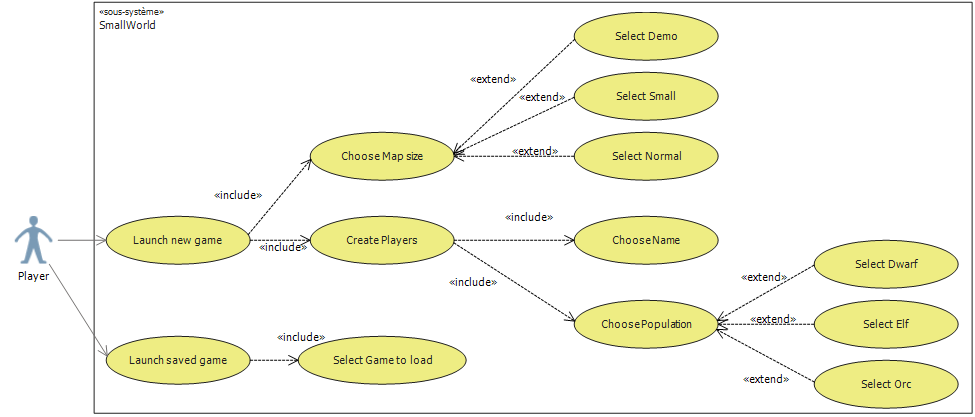
\includegraphics[width=18cm]{img/Diagramme_cas_utilisation_Creation.png}} 
    \caption{Diagramme de cas d'utilisation pour le lancement d'une partie} 
    \label{usecasecreate} 
  \end{center}
\end{figure}

\subsection{Cas du déroulement d'un tour}

Lorsque l’utilisateur est en train de jouer, plusieurs options s’offrent à lui (figure \ref{usecaseround}) :

\begin{itemize}\renewcommand{\labelitemi}{$\bullet$}
	\item Il peut sauvegarder sa partie en cours pour pouvoir la continuer ultérieurement.
    \item Il peut abandonner le jeu à tout moment.
    \item Il peut effectuer des actions avec ses unités. Pour cela, il devra cliquer sur l’unité qui l’interesse ainsi qu’une case adjacente puis valider son action. Si la case n’est pas occupée par une unité ennemie, l’unité se déplacera sur celle-ci. Dans le cas contraire, un combat sera engagé.
\end{itemize}

\begin{figure}[!h] 
  \begin{center}
    \makebox[\textwidth]{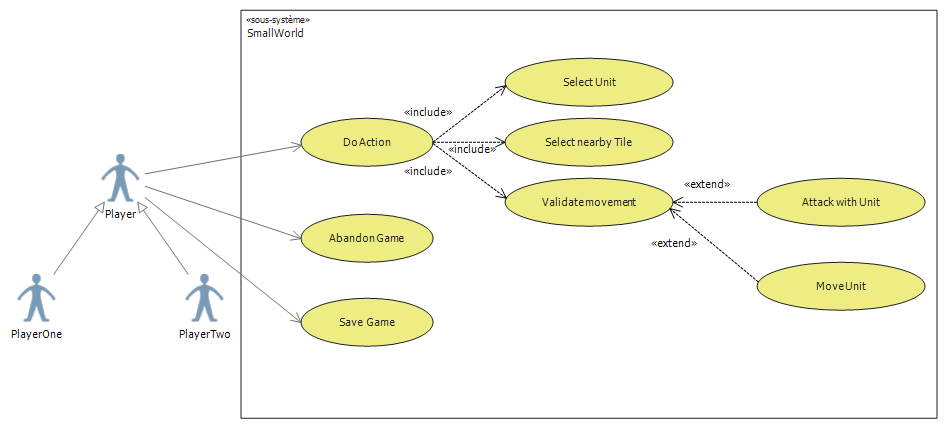
\includegraphics[width=18cm]{img/Diagramme_cas_utilisation_Round.png}} 
    \caption{Diagramme de cas d'utilisation pour le déroulement d'un tour} 
    \label{usecaseround} 
  \end{center}
\end{figure}

\newpage

\section{Diagrammes d’états-transitions}

\subsection{Cycle de vie du jeu}

Lorsqu’une nouvelle partie est créée, le jeu est “en cours”. Plusieurs transitions sont possibles (figure \ref{etattransjeu}) :
\begin{itemize}\renewcommand{\labelitemi}{$\bullet$}
	\item L’utilisateur quitte la partie. Dans ce cas, le jeu se termine.
	\item Un seul joueur est en vie. Cela signifie qu’un des deux joueurs ne possède plus d’unité en vie. Le jeu se termine également.
	\item Chaque type de carte possède un nombre de tours maximum. Si ce nombre est atteint alors le jeu se termine sinon il reste dans l’état “en cours”.
\end{itemize}

\begin{figure}[!h] 
  \begin{center}
    \makebox[\textwidth]{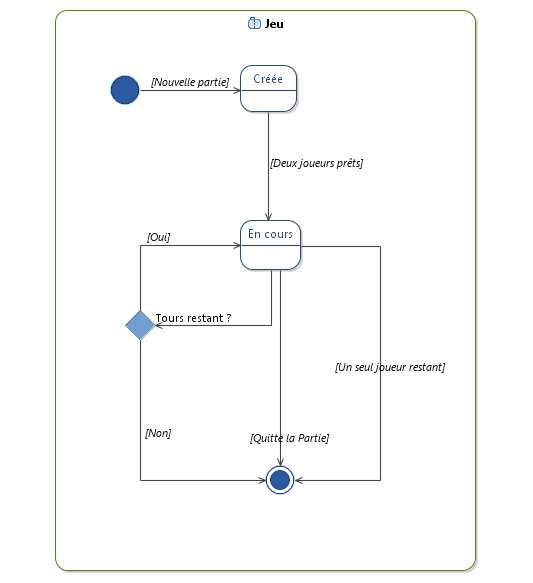
\includegraphics[width=12cm]{img/Diagramme_etatsTransitions_Jeu.png}} 
    \caption{Diagramme d'etats-transitions pour le Jeu} 
    \label{etattransjeu} 
  \end{center}
\end{figure}

\subsection{Cycle de vie d’une unité}

Lorsqu’une nouvelle partie est créée, l’unité est “au repos”. Plusieurs transitions sont possibles (figure \ref{etattransunite}) :
\begin{itemize}\renewcommand{\labelitemi}{$\bullet$}
	\item L’unité peut lancer une attaque ou se faire attaquer. Dans ces deux cas, on devra vérifier que l’unité est toujours en vie. Si tel est le cas, l’unité retourne dans l’état “au repos” sinon elle meurt.
	\item L’unité peut se déplacer. Dans ce cas précis, il n’y a pas de vérification à faire au niveau des points de vie de l’unité, elle reste dans l’état “au repos”.
	\item L’unité meurt également lorsque la partie se termine.
\end{itemize}

\begin{figure}[!h] 
  \begin{center}
    \makebox[\textwidth]{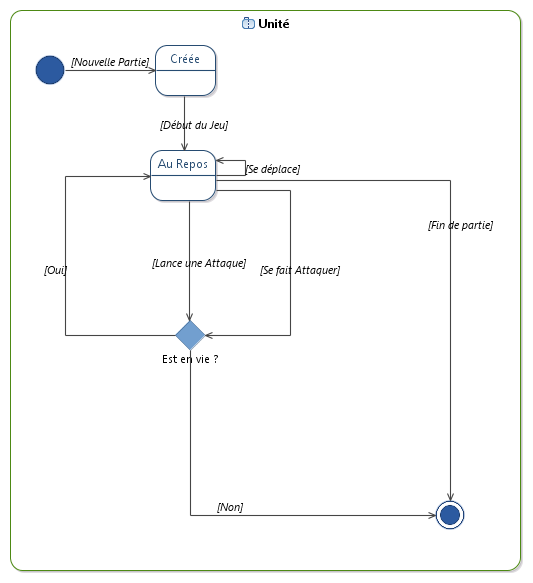
\includegraphics[width=10cm]{img/Diagramme_etatsTransitions_Unite.png}} 
    \caption{Diagramme d'etats-transitions pour une unité} 
    \label{etattransunite} 
  \end{center}
\end{figure}

\newpage

\section{Diagrammes d’interaction}
 
\subsection{Création d’une partie}

Lorsque l’utilisateur souhaite créer une partie, il va donner toutes les informations au «BuilderGame» : le type de carte, le nom du Joueur1, le type du peuple du Joueur1, le nom du Joueur2, le type du peuple du Joueur2 (figure \ref{sequencecreation}).

Le «BuilderGame» va ensuite pouvoir créer les joueurs grâce aux informations fournies. Il va aussi générer les unités en fonction des peuples choisis par l’utilisateur.
De plus, il s’occupe de créer la carte. En fonction du paramètre entré par l’utilisateur, on effectuera des boucles de différentes tailles (on peut le voir sur le diagramme grâce au cadre d’interaction «alt») :
\begin{itemize}\renewcommand{\labelitemi}{$\bullet$}
	\item Pour la carte Demo, la taille étant de 6 cases x 6 cases, on effectuera une boucle exécutée 36 fois afin de créer toutes les cases de la carte.
	\item Pour la carte Petite, de taille 10 cases x 10 cases, on effectuera la boucle 100 fois.
  	\item Pour la carte Normale, de taille 14 cases x 14 cases, on effectuera la boucle 196 fois.
\end{itemize}
Une fois les unités créées, elles seront positionnées sur la carte puis la partie sera lancée.

\begin{figure}[!h] 
  \begin{center}
    \makebox[\textwidth]{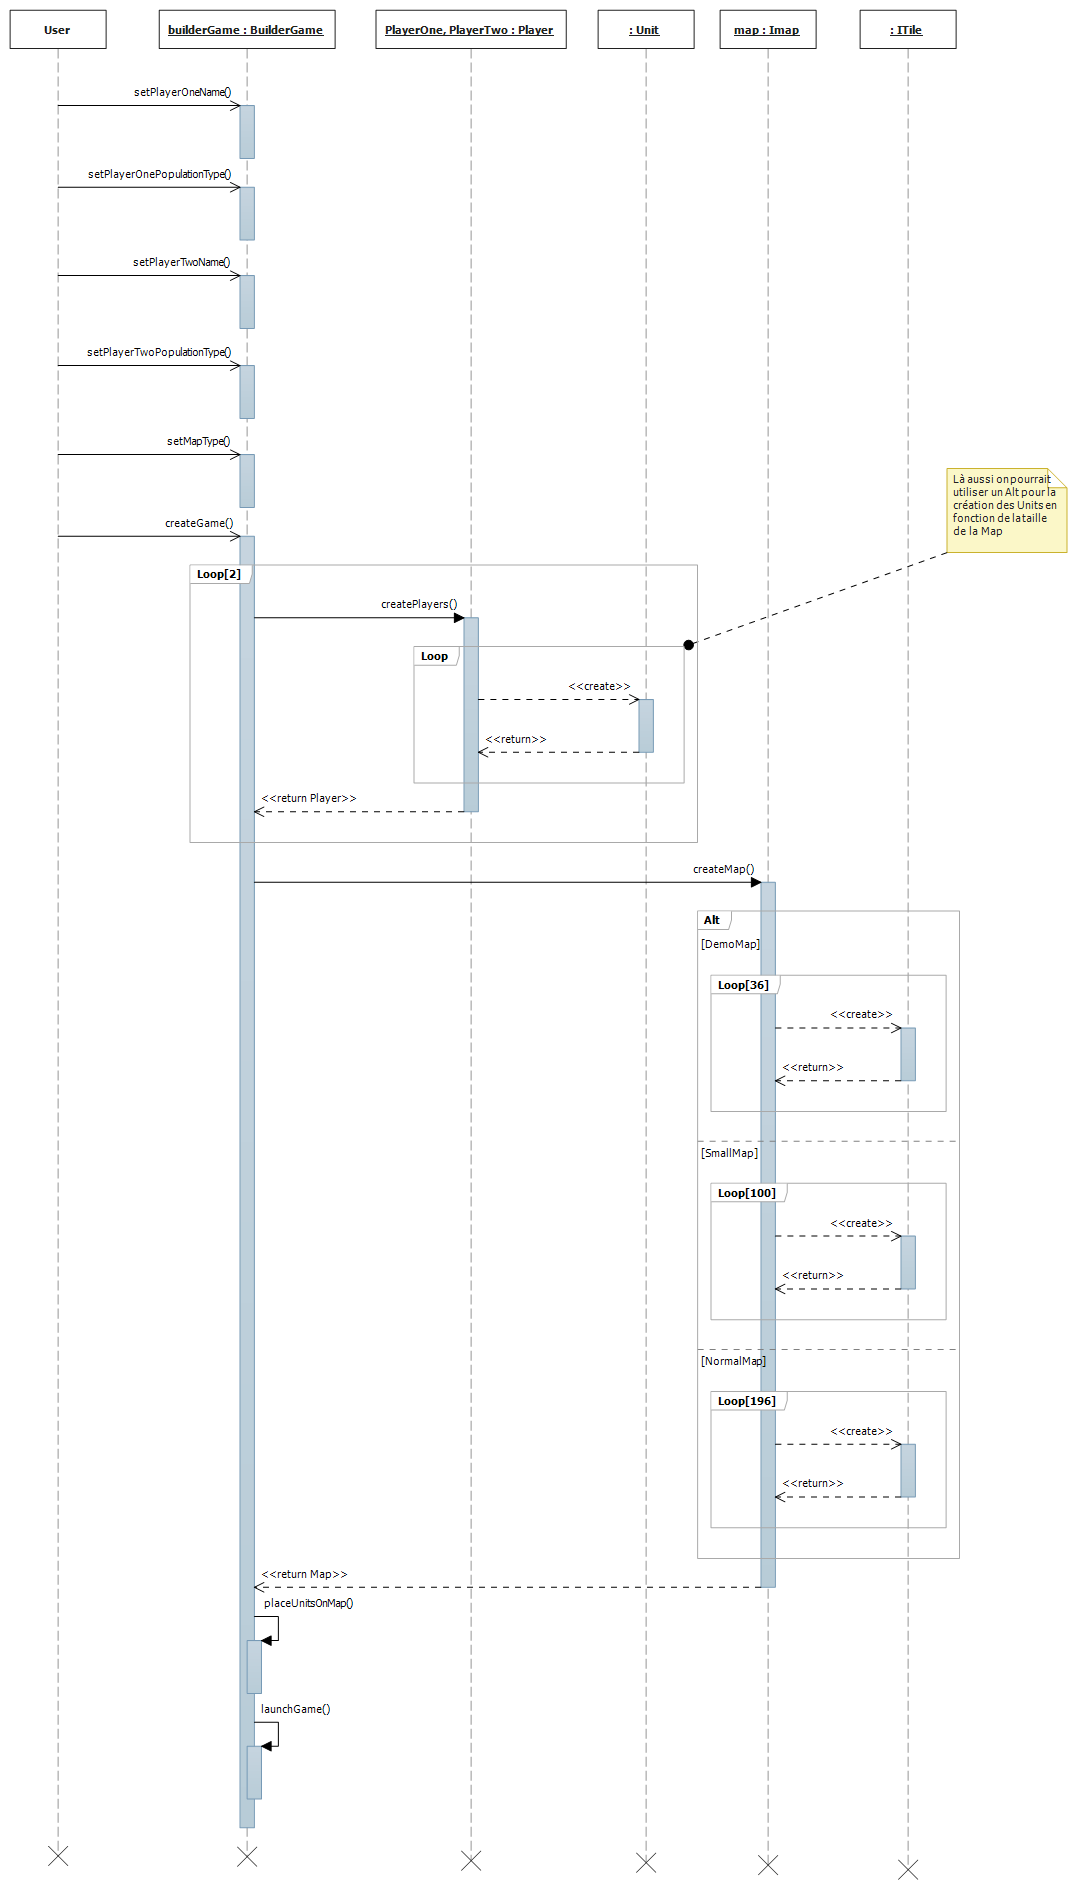
\includegraphics[width=10.5cm]{img/Diagramme_de_sequence_Creation.png}} 
    \caption{Diagramme de séquence pour la création d'une partie} 
    \label{sequencecreation} 
  \end{center}
\end{figure}

\subsection{Déroulement d’un tour pour un joueur}

Pour réaliser son tour, un joueur aura la possibilité d’effectuer des actions tant que ses unités sont en vie et avec des points de déplacement (figure \ref{sequenceround}). Pour réaliser une action, le joueur devra sélectionner l’une de ses unités ainsi qu’une case adjacente puis valider l’action. Si un ennemi est présent sur la case, il sera attaqué par l’unité précédemment sélectionnée. Si la case est vide, l’unité se déplacera.

Après chaque action, le score des joueurs sera actualisé pour qu’il puisse en tenir compte.
    
Si le joueur ne souhaite pas bouger l’une de ses unités pendant l’un de ses tours, il lui suffira de ne pas la sélectionner.



\begin{figure}[!h] 
  \begin{center}
    \makebox[\textwidth]{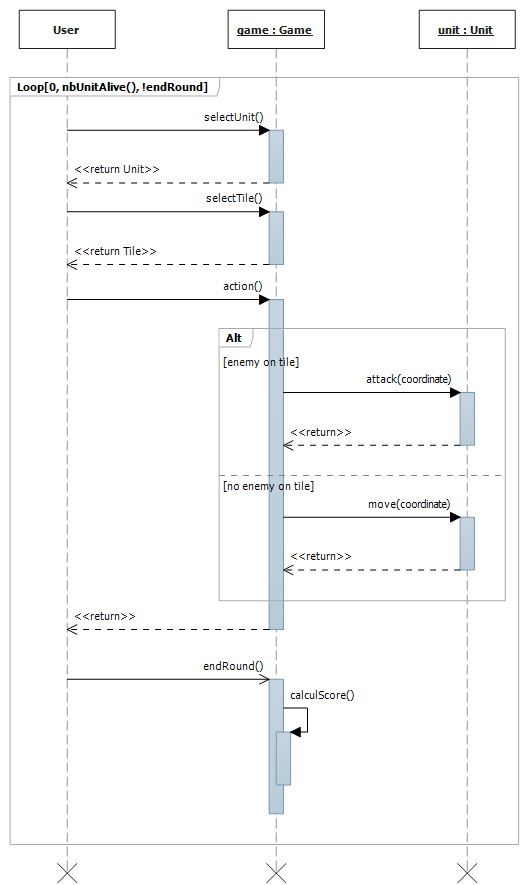
\includegraphics[width=8cm]{img/Diagramme_de_sequence_Round.png}} 
    \caption{Diagramme de séquence pour le déroulement d'un tour} 
    \label{sequenceround} 
  \end{center}
\end{figure}

\newpage

\section{Diagrammes de classe}

Dans cette partie nous allons présenter les différents patrons de conception que nous avons utilisés pour le diagramme de classe.

\subsection{Fabrique pour gérer les différents peuples}

Pour générer les différents peuples, nous utilisons une Fabrique (figure \ref{fabrique}). Ce motif de conception est utilisé lorsqu’à l’exécution il est nécessaire de déterminer quel objet d’un ensemble de sous classe doit être instancier. Dans notre cas, il faut choisir entre les trois peuples elf, orc ou nain.

\begin{figure}[!h] 
  \begin{center}
    \makebox[\textwidth]{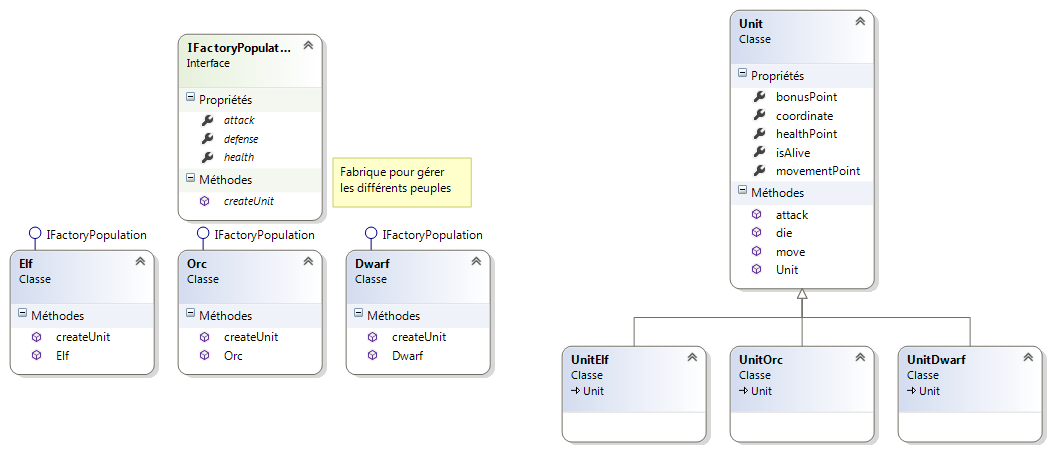
\includegraphics[width=14cm]{img/fabrique.png}} 
    \caption{Fabrique pour gérer les différents peuples} 
    \label{fabrique} 
  \end{center}
\end{figure}


\subsection{Monteur pour la création d’une partie}

Nous utilisons un Monteur (figure \ref{monteur}) pour la création d’une partie car la construction de certains objets qui la composent peut être complexe. Le monteur nous permet donc de séparer les différentes étapes de création et de les ordonner. Il nous permettra aussi de gérer les différents types de partie que l’on veut lancer : le choix entre créer une nouvelle partie ou charger une partie sauvegardée.

\begin{figure}[!h] 
  \begin{center}
    \makebox[\textwidth]{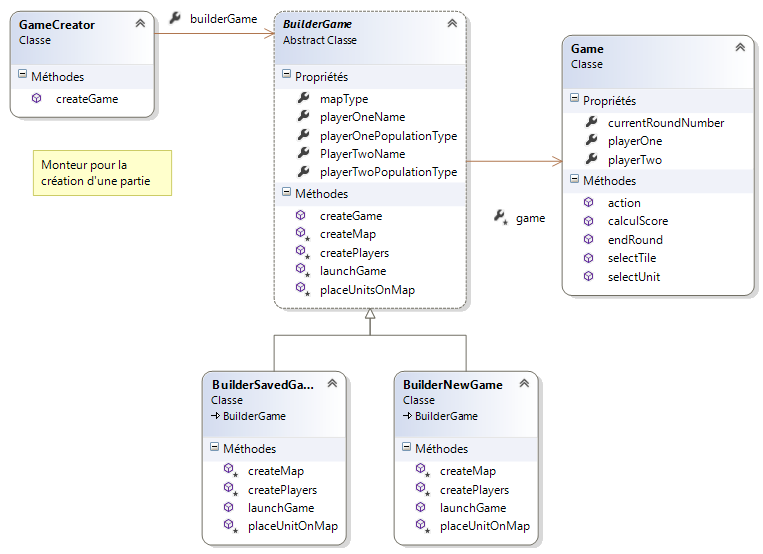
\includegraphics[width=10cm]{img/monteur.png}} 
    \caption{Monteur pour la création d’une partie} 
    \label{monteur} 
  \end{center}
\end{figure}

\subsection{Poids-Mouche pour la modélisation de la carte}

Pour la génération de la carte, nous devons utiliser un Poids-Mouche (figure \ref{poidsMouche}). En effet, la carte est composée de très nombreuses cases qui, si on devait toutes les instancier, serait  très gourmandes en mémoire. Ce patron de conception nous permet de n’instancier qu’une seule fois les types de cases, et de les réutiliser dès qu’on en a le besoin. Cela permet au final d’alléger la mémoire.

\begin{figure}[!h] 
  \begin{center}
    \makebox[\textwidth]{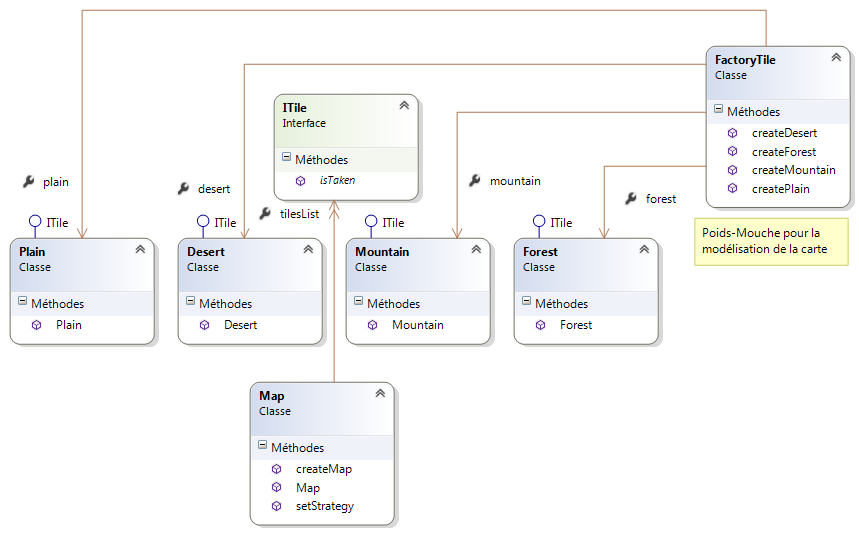
\includegraphics[width=13cm]{img/poidsMouche.png}} 
    \caption{Poids-Mouche pour la modélisation de la carte} 
    \label{poidsMouche} 
  \end{center}
\end{figure}

\subsection{Stratégie pour la création des différents types de carte}

L’utilisateur, à la création de la partie, peut choisir entre trois types de carte (Demo, Petite, Normale). C’est au rôle de la Stratégie (figure \ref{strategie}) de définir le comportement de création de la carte en fonction du contexte et du choix utilisateur.

\begin{figure}[!h] 
  \begin{center}
    \makebox[\textwidth]{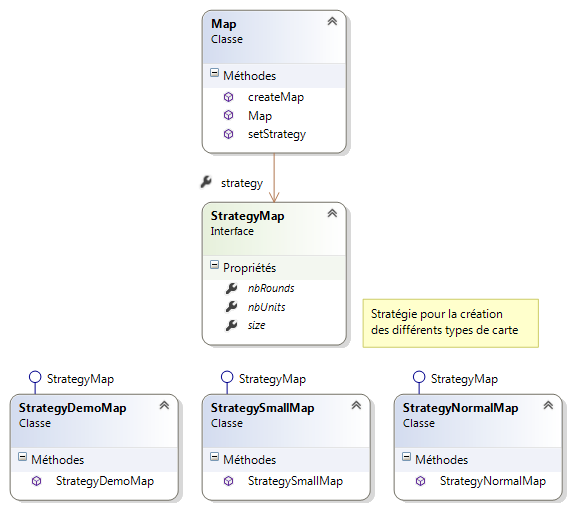
\includegraphics[width=10cm]{img/strategie.png}} 
    \caption{Stratégie pour la création des différents types de carte} 
    \label{strategie} 
  \end{center}
\end{figure}

\subsection{Diagramme de classe global}

Pour une visualisation complète de notre modélisation, voici en figure \ref{global} notre diagramme de classe.

\newpage

\thispagestyle{plain}
\begin{figure}[!h] 
  \begin{center}
    \makebox[\textwidth]{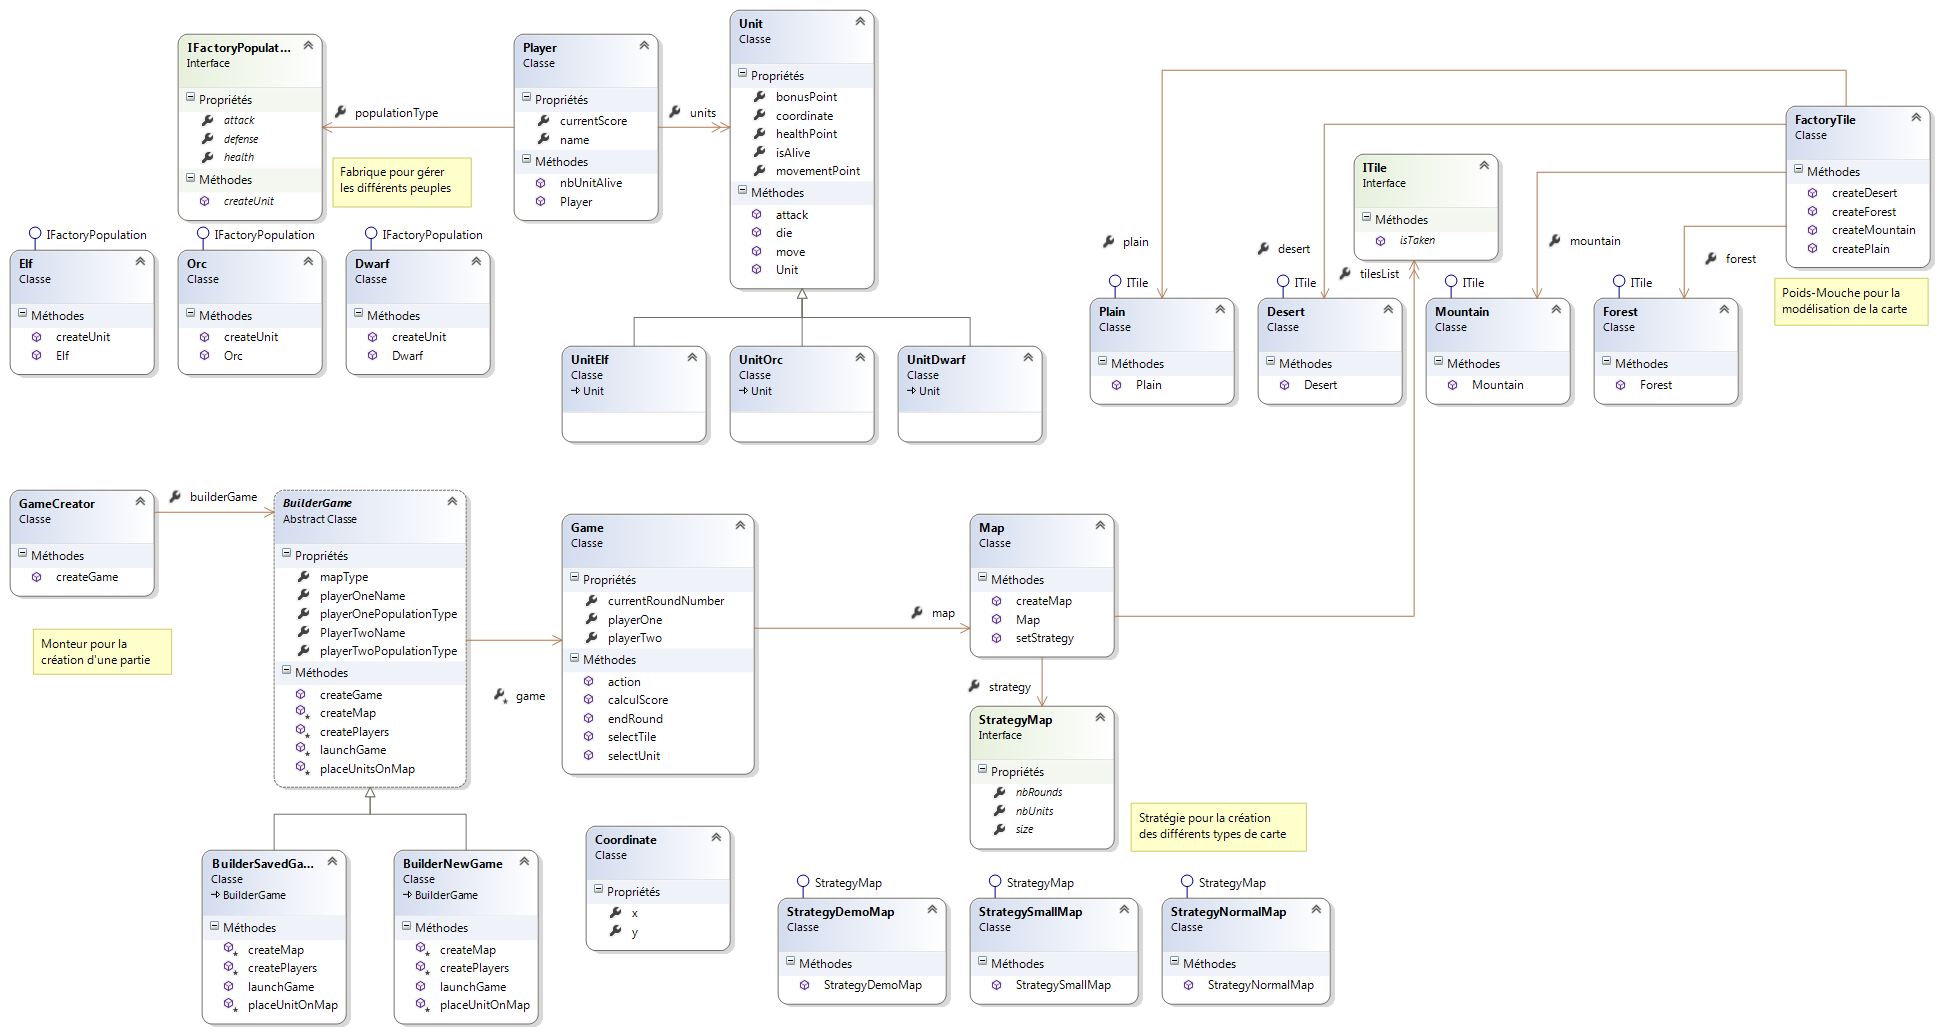
\includegraphics[angle=90,width=11cm]{img/Diagramme_de_classe.png}} 
    \caption{Diagramme de classe global} 
    \label{global2} 
  \end{center}
\end{figure}


\end{document}